Along with the implementation of the proof-of-concept, multiple experiments were conducted to evaluate the networking and computational performance of the proposed approach. The testbed was empirically hosted on a laptop with an AMD Ryzen 7 4700U CPU and 16 GB of RAM, running an x86-64 Linux 6.1.24-1-lts system. Every instance got assigned 1 GB of RAM and 2 virtual CPUs. 

The bridge interface, pooling all the mesh traffic exchanged between the tap interfaces, was the starting point for the networking measurements. All these interfaces had a maximum virtual bandwidth of 10 Mbit per second, assigned by the hosting system. The traffic was monitored using Wireshark\footnote{\url{https://www.wireshark.org/}}, and the metrics were collected throughout the various stages of the experiment, by listening to packets of different kinds, flowing through the bridge interface. Establishing the mesh network connectivity, the Ethernet frames belonging to the batman-adv protocol sized an average of 74 bytes, and the IPv4 related packets averaged at 278 bytes, presenting both protocols a seemingly linear throughput increase with the increase in the number of instances, as shown in Figure~\ref{fig:mesh-traffic}. 

\begin{figure} [h!]
    \centering
    \begin{subfigure}[b]{0.49\textwidth}
        \centering
        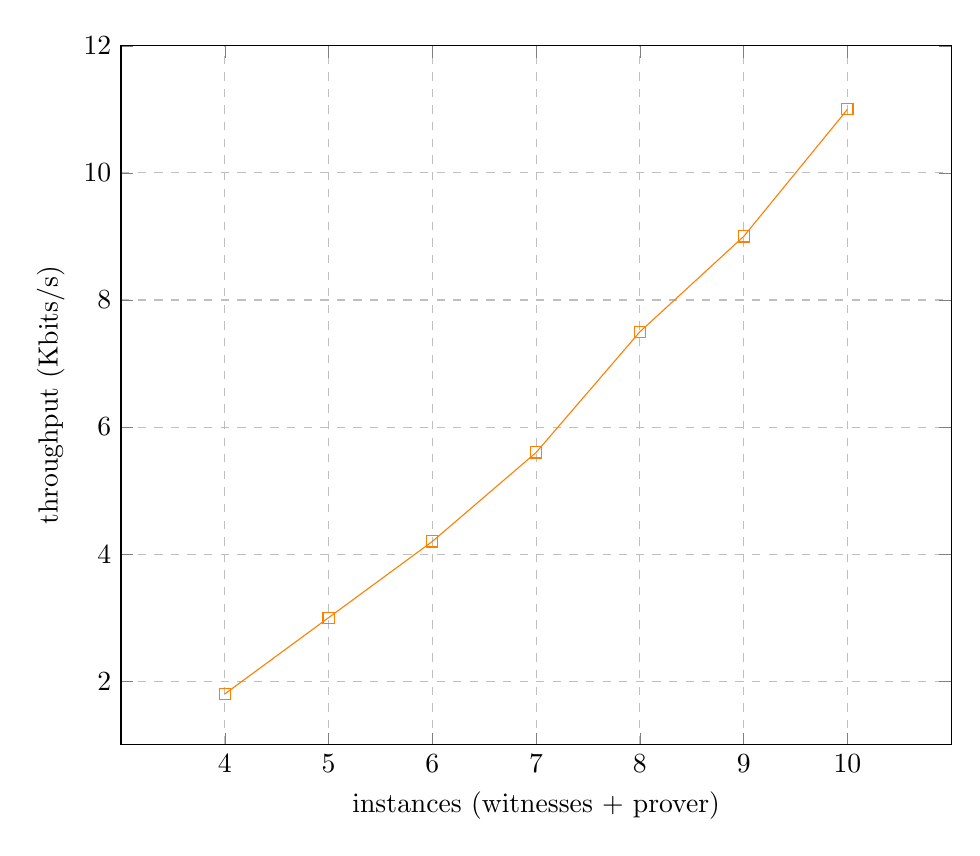
\begin{tikzpicture}
            \definecolor{line-color}{RGB}{92,255,230}
            \definecolor{line-color2}{RGB}{3,150,156}
            \begin{axis}[
                legend pos=outer north east,
                xlabel=instances (witnesses + prover),
                ylabel=throughput (Kbits/s),
                xmin=3, xmax=11,
                ymin=1, ymax=12,
                xtick={4,5,6,7,8,9,10},
                ytick={2, 4, 6, 8, 10, 12},
                grid=major,
                grid style={dashed},
                width=\textwidth
            ]
            
            \addplot[color=orange,mark=square] coordinates {
                (4,1.8) (5,3.0) (6,4.2) (7,5.6) (8,7.5) (9,9.0) (10,11)
                % (4,3.4) (5,5.7) (6,8.1) (7,11.2) (8,14) (9,16.8) (10,20)
            };
            \end{axis}
        \end{tikzpicture}
        \caption{Batman-adv traffic throughput.}
        \label{fig:y equals x}
    \end{subfigure}
    \hfill
    \begin{subfigure}[b]{0.49\textwidth}
        \centering
        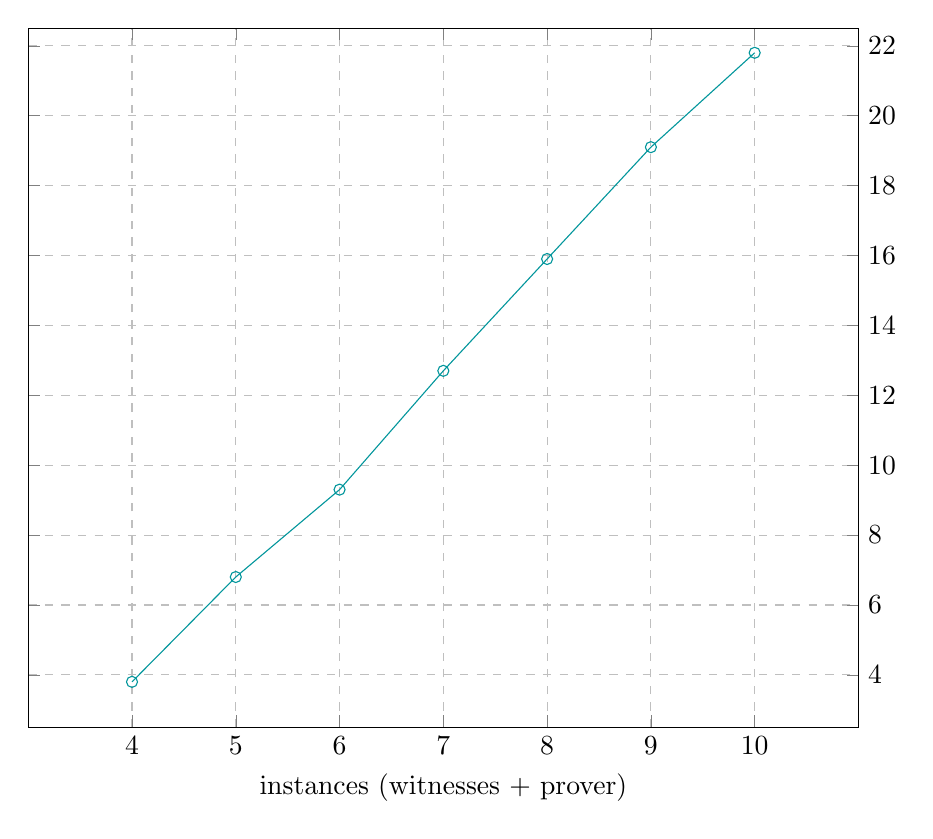
\begin{tikzpicture}
            \definecolor{line-color}{RGB}{92,255,230}
            \definecolor{line-color2}{RGB}{3,150,156}
            \begin{axis}[
                legend pos=outer north east,
                xlabel=instances (witnesses + prover),
                % ylabel=throughput (Kbits/s),
                yticklabel pos=right,
                xmin=3, xmax=11,
                ymin=2.5, ymax=22.5,
                xtick={4,5,6,7,8,9,10},
                ytick={2, 4, 6, 8, 10, 12, 14, 16, 18, 20, 22},
                grid=major,
                grid style={dashed},
                width=\textwidth,
            ]
            
            \addplot[color=line-color2,mark=o] coordinates {
                (4,3.8) (5,6.8) (6,9.3) (7,12.7) (8,15.9) (9,19.1) (10,21.8)
            };        
            \end{axis}
        \end{tikzpicture}
        \caption{IPv4 traffic throughput.}
        \label{fig:three sin x}
    \end{subfigure}
    \caption{Average protocol throughput, measured on the bridge interface.}
    \label{fig:mesh-traffic}
\end{figure}

The Blockchain activity was also monitored, in order to observe the protocol behaviour, regarding the block generation and proposal phases. Figure~\ref{fig:blockchain-blocks-generation} captures the number of messages exchanged between the instances, during a time frame of typical protocol activity. The interval time between blocks, set to 10 seconds, corresponds to the higher peaks of TCP traffic, while the UDP traffic is more evenly distributed.

\begin{figure}[h!]
\pgfplotstableread[col sep=comma]{data/blockchain-blocks-generation.csv}\datatable

\begin{tikzpicture}
    \definecolor{line-color}{RGB}{3,150,156}
    \definecolor{line-color2}{RGB}{167,169,172}
    \begin{axis}[
        xlabel=time (s),
        ylabel=messages,
        xmin=-2, xmax=102,
        ymin=-50, ymax=300,
        ytick={0, 50, 100, 150, 200, 250, 300},
        grid=major,
        grid style={dashed},
        width=\textwidth,
        height=0.5\textwidth,
        legend pos=north west
    ]

    \addplot[mark=*,line-color] table[x=x,y=TCP]{\datatable};
    \addplot[mark=+,line-color2] table[x=x,y=UDP]{\datatable};
    \addplot[mark=o,red] table[x=x,y=Batman-adv-orig]{\datatable};

    \legend{TCP, UDP, Batman-adv-orig}

    \end{axis}
\end{tikzpicture}
\caption{The network activity, with a block time of 10 seconds.}
\label{fig:blockchain-blocks-generation}
\end{figure}

Both CPU and RAM usage were also continuously measured across the whole experiment. The two virtual cores of each instance saw the CPU usage averaging at 2\%, peaking at 20\% when a witness would interact with the prover, in order to produce a \pol{} certificate. The overall RAM usage did not go beyond 200 MB. These numbers are in line with the expected behaviour of the protocol, running the PoA consensus algorithm, as a lightweight mechanism that may not require much computational power, suitable and adaptable to resource-constrained environments. The PoW consensus algorithm, on the other hand, would require a much higher and variable computational power, that would be difficult to predict and control, as it is not only manually configured, but dependent, as well, on the dynamic difficulty adjustment mechanism, in order to meet a fixed block time.

\TODO{I am thinking of completing one more experiment: Changing the block time interval and measure the failure rate of the generation of \pol{} certificates... This would show the effect of the block time on tackling the proxy attacks. What do you think? It shall result in an inverse relationship between the block time and the failure rate of the \pol{} certificates. The higher the block time, the lower the failure rate.}

% \begin{figure}[h!]
%     \begin{center}
% \begin{tikzpicture}
%     \definecolor{line-color}{RGB}{92,255,230}
%     \definecolor{line-color2}{RGB}{3,150,156}
%     \begin{axis}[
%         legend pos=outer north east,
%         xlabel=number of instances (witnesses + prover),
%         ylabel=throughput (Kbits/s),
%         xmin=3, xmax=11,
%         ymin=1, ymax=12,
%         xtick={4,5,6,7,8,9,10},
%         ytick={2, 4, 6, 8, 10, 12},
%         grid=major,
%         grid style={dashed},
%         width=0.8\textwidth,
%         height=0.4\textwidth,
%     ]
    
%     \addplot[color=orange,mark=square] coordinates {
%         (4,1.8) (5,3.0) (6,4.2) (7,5.6) (8,7.5) (9,9.0) (10,11)
%         % (4,3.4) (5,5.7) (6,8.1) (7,11.2) (8,14) (9,16.8) (10,20)
%     };
%     % \addlegendentry{batman-adv}

%     % \addplot[color=line-color2,mark=o] coordinates {
%     %     (4,4.5) (5,6.8) (6,9.3) (7,12.7) (8,15.9) (9,19.1) (10,21.8)
%     % };
%     % \addlegendentry{IPv4}

%     \end{axis}
% \end{tikzpicture}
% \caption{Average batman-adv traffic throughput, measured on the bridge interface.}
% \label{fig:mesh-traffic}
% \end{center}
% \end{figure}

% \begin{figure}[h!]
%     \begin{center}
% \begin{tikzpicture}
%     \definecolor{line-color}{RGB}{92,255,230}
%     \definecolor{line-color2}{RGB}{3,150,156}
%     \begin{axis}[
%         legend pos=outer north east,
%         xlabel=number of instances (witnesses + prover),
%         ylabel=throughput (Kbits/s),
%         xmin=3, xmax=11,
%         ymin=2.5, ymax=22.5,
%         xtick={4,5,6,7,8,9,10},
%         ytick={2, 4, 6, 8, 10, 12, 14, 16, 18, 20, 22},
%         grid=major,
%         grid style={dashed},
%         width=0.8\textwidth,
%         height=0.4\textwidth,
%     ]
    
%     \addplot[color=line-color2,mark=o] coordinates {
%         (4,4.5) (5,6.8) (6,9.3) (7,12.7) (8,15.9) (9,19.1) (10,21.8)
%     };
%     \addlegendentry{IPv4}

%     \end{axis}
% \end{tikzpicture}
% \caption{Average batman-adv traffic throughput, measured on the bridge interface.}
% \label{fig:mesh-traffic}
% \end{center}
% \end{figure}

% \begin{figure} [h!]
% \begin{tabular}{c c}
% \begin{minipage}{0.50\textwidth}
%     \begin{center}
%         \begin{tikzpicture}
%             \definecolor{line-color}{RGB}{92,255,230}
%             \definecolor{line-color2}{RGB}{3,150,156}
%             \begin{axis}[
%                 legend pos=outer north east,
%                 xlabel=instances (witnesses + prover),
%                 ylabel=throughput (Kbits/s),
%                 xmin=3, xmax=11,
%                 ymin=1, ymax=12,
%                 xtick={4,5,6,7,8,9,10},
%                 ytick={2, 4, 6, 8, 10, 12},
%                 grid=major,
%                 grid style={dashed},
%                 width=\textwidth,
%                 height=0.8\textwidth,
%             ]
            
%             \addplot[color=orange,mark=square] coordinates {
%                 (4,1.8) (5,3.0) (6,4.2) (7,5.6) (8,7.5) (9,9.0) (10,11)
%                 % (4,3.4) (5,5.7) (6,8.1) (7,11.2) (8,14) (9,16.8) (10,20)
%             };
%             \end{axis}
%         \end{tikzpicture}
%         \caption{(a) Average batman-adv traffic throughput.}
%         % \label{fig:mesh-traffic}
%         \end{center}
% \end{minipage}
% &
% \begin{minipage}{0.50\textwidth}

%     \begin{center}
%         \begin{tikzpicture}
%             \definecolor{line-color}{RGB}{92,255,230}
%             \definecolor{line-color2}{RGB}{3,150,156}
%             \begin{axis}[
%                 legend pos=outer north east,
%                 xlabel=instances (witnesses + prover),
%                 % ylabel=throughput (Kbits/s),
%                 xmin=3, xmax=11,
%                 ymin=2.5, ymax=22.5,
%                 xtick={4,5,6,7,8,9,10},
%                 ytick={2, 4, 6, 8, 10, 12, 14, 16, 18, 20, 22},
%                 grid=major,
%                 grid style={dashed},
%                 width=\textwidth,
%                 height=0.8\textwidth,
%             ]
            
%             \addplot[color=line-color2,mark=o] coordinates {
%                 (4,4.5) (5,6.8) (6,9.3) (7,12.7) (8,15.9) (9,19.1) (10,21.8)
%             };        
%             \end{axis}
%         \end{tikzpicture}
%         \caption{(a) Average IPv4 traffic throughput.}
%         \end{center}

% \end{minipage}
% \end{tabular}
% \caption{Example how to put two figures parallel to each other.}
% \label{fig:LCA_2_solutions}
% \end{figure}

% \begin{figure}[h!]
% \pgfplotstableread[col sep=comma]{data/br-qemu.csv}\datatable

% \begin{tikzpicture}
%     \definecolor{line-color}{RGB}{3,150,156}
%     \definecolor{line-color2}{RGB}{167,169,172}
%     \begin{axis}[
%         xlabel=time (s),
%         ylabel=throughput (Bits/s),
%         xmin=10, xmax=20,
%         ymin=-100, ymax=1300,
%         ytick={0,200,400,600,800,1000,1200},
%         grid=major,
%         grid style={dashed},
%         width=\textwidth,
%         height=0.5\textwidth,
%     ]

%     \addplot[mark=*,line-color2] table[x=Interval start,y=prover 1]{\datatable};
%     \addplot[mark=+,line-color] table[x=Interval start,y=witness 1]{\datatable};
%     \addplot[mark=x,line-color] table[x=Interval start,y=witness 2]{\datatable};
%     \addplot[mark=o,line-color] table[x=Interval start,y=witness 3]{\datatable};

%     \legend{prover, witness 1, witness 2, witness 3}

%     \end{axis}
% \end{tikzpicture}
% \caption{Ethernet traffic throughput, measured on the bridge interface.}
% \label{fig:mesh-traffic-3-witnesses}
% \end{figure}



% AMD Ryzen 7 4700U with Radeon Graphics (with SSE4.2)
% Linux 6.1.24-1-lts
